%%
%% This is file `acmsmall-submission.tex',
%% generated with the docstrip utility.
%%
%% The original source files were:
%%
%% samples.dtx  (with options: `all,acmsmall,submission')
%% 
%% IMPORTANT NOTICE:
%% 
%% For the copyright see the source file.
%% 
%% Any modified versions of this file must be renamed
%% with new filenames distinct from acmsmall-submission.tex.
%% 
%% For distribution of the original source see the terms
%% for copying and modification in the file samples.dtx.
%% 
%% This generated file may be distributed as long as the
%% original source files, as listed above, are part of the
%% same distribution. (The sources need not necessarily be
%% in the same archive or directory.)
%%
%%
%% Commands for TeXCount
%TC:macro \cite [option:text,text]
%TC:macro \citep [option:text,text]
%TC:macro \citet [option:text,text]
%TC:envir table 0 1
%TC:envir table* 0 1
%TC:envir tabular [ignore] word
%TC:envir displaymath 0 word
%TC:envir math 0 word
%TC:envir comment 0 0
%%
%% The first command in your LaTeX source must be the \documentclass
%% command.
%%
%% For submission and review of your manuscript please change the
%% command to \documentclass[manuscript, screen, review]{acmart}.
%%
%% When submitting camera ready or to TAPS, please change the command
%% to \documentclass[sigconf]{acmart} or whichever template is required
%% for your publication.
%%
%%

\documentclass[acmsmall,screen,anonymous,review]{acmart}
%%
%% \BibTeX command to typeset BibTeX logo in the docs
\AtBeginDocument{%
  \providecommand\BibTeX{{%
    Bib\TeX}}}

%% Rights management information.  This information is sent to you
%% when you complete the rights form.  These commands have SAMPLE
%% values in them; it is your responsibility as an author to replace
%% the commands and values with those provided to you when you
%% complete the rights form.
\setcopyright{acmlicensed}
\copyrightyear{2018}
\acmYear{2018}
\acmDOI{XXXXXXX.XXXXXXX}

%% These commands are for a JOURNAL article.
\acmJournal{JACM}
\acmVolume{37}
\acmNumber{4}
\acmArticle{111}
\acmMonth{8}

%%
%% Submission ID.
%% Use this when submitting an article to a sponsored event. You'll
%% receive a unique submission ID from the organizers
%% of the event, and this ID should be used as the parameter to this command.
%%\acmSubmissionID{123-A56-BU3}

%%
%% For managing citations, it is recommended to use bibliography
%% files in BibTeX format.
%%
%% You can then either use BibTeX with the ACM-Reference-Format style,
%% or BibLaTeX with the acmnumeric or acmauthoryear sytles, that include
%% support for advanced citation of software artefact from the
%% biblatex-software package, also separately available on CTAN.
%%
%% Look at the sample-*-biblatex.tex files for templates showcasing
%% the biblatex styles.
%%
%%
%% The majority of ACM publications use numbered citations and
%% references.  The command \citestyle{authoryear} switches to the
%% "author year" style.
%%
%% If you are preparing content for an event
%% sponsored by ACM SIGGRAPH, you must use the "author year" style of
%% citations and references.
%% Uncommenting
%% the next command will enable that style.
%%\citestyle{acmauthoryear}

\usepackage{tikz}
\usetikzlibrary{arrows.meta,positioning,shapes.geometric}

\tikzset{
  flowinput/.style={
    rectangle, rounded corners=2pt, draw=blue!60!black, fill=blue!8,
    align=center, text width=5.2cm, minimum height=9mm
  },
  flowstep/.style={
    rectangle, rounded corners=2pt, draw=black!70, fill=gray!8,
    align=center, text width=5.2cm, minimum height=9mm
  },
  flowoutput/.style={
    rectangle, rounded corners=2pt, draw=green!50!black, fill=green!10,
    align=center, text width=5.2cm, minimum height=9mm
  },
  flowdecision/.style={
    diamond, draw=orange!80!black, fill=orange!10, align=center,
    aspect=2, inner sep=1.5pt, text width=2.3cm
  },
  flowarrow/.style={-{Stealth[length=2mm]}, thick}
}

%%
%% end of the preamble, start of the body of the document source.
\begin{document}

%%
%% The "title" command has an optional parameter,
%% allowing the author to define a "short title" to be used in page headers.
\title{The Name of the Title Is Hope}

%%
%% The "author" command and its associated commands are used to define
%% the authors and their affiliations.
%% Of note is the shared affiliation of the first two authors, and the
%% "authornote" and "authornotemark" commands
%% used to denote shared contribution to the research.
\author{Ben Trovato}
\authornote{Both authors contributed equally to this research.}
\email{trovato@corporation.com}
\orcid{1234-5678-9012}
\author{G.K.M. Tobin}
\correspondingauthor
\authornotemark[1]
\email{webmaster@marysville-ohio.com}
\affiliation{%
  \institution{Institute for Clarity in Documentation}
  \city{Dublin}
  \state{Ohio}
  \country{USA}
}

\author{Lars Th{\o}rv{\"a}ld}
\affiliation{%
  \institution{The Th{\o}rv{\"a}ld Group}
  \city{Hekla}
  \country{Iceland}}
\email{larst@affiliation.org}

\author{Valerie B\'eranger}
\affiliation{%
  \institution{Inria Paris-Rocquencourt}
  \city{Rocquencourt}
  \country{France}
}

\author{Aparna Patel}
\affiliation{%
 \institution{Rajiv Gandhi University}
 \city{Doimukh}
 \state{Arunachal Pradesh}
 \country{India}}

\author{Huifen Chan}
\affiliation{%
  \institution{Tsinghua University}
  \city{Haidian Qu}
  \state{Beijing Shi}
  \country{China}}

\author{Charles Palmer}
\affiliation{%
  \institution{Palmer Research Laboratories}
  \city{San Antonio}
  \state{Texas}
  \country{USA}}
\email{cpalmer@prl.com}

\author{John Smith}
\affiliation{%
  \institution{The Th{\o}rv{\"a}ld Group}
  \city{Hekla}
  \country{Iceland}}
\email{jsmith@affiliation.org}

\author{Julius P. Kumquat}
\correspondingauthor
\affiliation{%
  \institution{The Kumquat Consortium}
  \city{New York}
  \country{USA}}
\email{jpkumquat@consortium.net}

%%
%% By default, the full list of authors will be used in the page
%% headers. Often, this list is too long, and will overlap
%% other information printed in the page headers. This command allows
%% the author to define a more concise list
%% of authors' names for this purpose.
\renewcommand{\shortauthors}{Trovato et al.}

%%
%% The abstract is a short summary of the work to be presented in the
%% article.
\begin{abstract}
  A clear and well-documented \LaTeX\ document is presented as an
  article formatted for publication by ACM in a conference proceedings
  or journal publication. Based on the ``acmart'' document class, this
  article presents and explains many of the common variations, as well
  as many of the formatting elements an author may use in the
  preparation of the documentation of their work.
\end{abstract}

%%
%% The code below is generated by the tool at http://dl.acm.org/ccs.cfm.
%% Please copy and paste the code instead of the example below.
%%

\ccsdesc[500]{Do Not Use This Code~Generate the Correct Terms for Your Paper}
\ccsdesc[300]{Do Not Use This Code~Generate the Correct Terms for Your Paper}
\ccsdesc{Do Not Use This Code~Generate the Correct Terms for Your Paper}
\ccsdesc[100]{Do Not Use This Code~Generate the Correct Terms for Your Paper}


\received{20 February 2007}
\received[revised]{12 March 2009}
\received[accepted]{5 June 2009}

%%
%% This command processes the author and affiliation and title
%% information and builds the first part of the formatted document.
\maketitle

\section{Introduction}

\section{Background and Related Work}

The decomposition of monolithic systems into microservice-oriented architectures has been investigated from different perspectives, including structural analysis of source code, information obtained during system execution, and, more recently, artificial intelligence techniques capable of incorporating semantic information into the process of identifying service boundaries. The increasing adoption of Large Language Models (LLMs) has expanded this research space by enabling architectural information expressed in natural language and implementation artifacts to be interpreted during software comprehension, architecture recovery, and architectural design activities. In this context, the works most closely related to this study can be organized into three main groups: decomposition approaches based on structural or behavioral information, approaches that employ LLMs to transform textual descriptions into architectural representations, and approaches that integrate LLMs with code analysis and architecture recovery or transformation.

\subsection{Decomposition Based on Structural and Behavioral Information}

Before the recent adoption of generative LLMs, different decomposition techniques sought to identify microservice candidates based on structural or behavioral characteristics of software systems. These approaches typically rely on dependencies among components, coupling and cohesion metrics, graphs, or information obtained from system execution to identify groups of related elements.

The MINDS framework, proposed by Ait Mansour et al., exemplifies an approach oriented toward system behavior. Rather than relying exclusively on static dependencies extracted from source code, the approach uses event logs and execution traces to identify activities associated with different business domains. Transformer-based models, particularly BERT, are employed to capture semantic information from recorded activities and support their classification into business-domain clusters. Process mining techniques are subsequently applied to support the identification of functional service boundaries.

The results reported for MINDS indicate that incorporating activity semantics can produce decompositions with high cohesion and relatively low coupling. However, the approach depends on the availability of execution information and on an appropriate event-logging pipeline. In legacy systems, such information may be incomplete or even unavailable. Furthermore, the method mainly focuses on functional decomposition and does not explicitly account for other architectural requirements and constraints.

These studies reveal an important shift from purely structural techniques: semantic information can complement software metrics when identifying microservice boundaries. Nevertheless, models such as BERT are primarily used as representation or classification mechanisms rather than as generative reasoning mechanisms for architectural decision-making. The recent development of LLMs therefore introduces new possibilities for incorporating domain descriptions, requirements, and architectural knowledge into decomposition activities.


\subsection{LLMs for Archuitectural Generation from Textual Descriptions}

A second research direction investigates the ability of LLMs to transform natural-language descriptions into architectural representations or decisions. Unlike approaches that rely on the existing implementation of a system, these studies mainly operate on requirements, functional descriptions, constraints, or project context.

Tagliaferro et al. investigated the automatic generation of UML component diagrams from informal specifications. In their approach, an LLM receives a textual system description and produces a corresponding PlantUML representation. The process relies on conventional prompting, with explicit instructions regarding the expected output structure and examples provided through in-context learning. In this way, the model acts directly on the transformation from requirements information to architectural representation.

Their experiments showed that the LLM was capable of producing syntactically valid diagrams and of correctly representing several elements explicitly mentioned in the specifications. However, the results also revealed difficulties in identifying implicit architectural concepts. Elements that required domain knowledge or additional inference were frequently omitted from the generated architecture. As a consequence, some solutions were excessively simplified or centralized.

Maranhão and Guerra explore another application of LLMs in architectural design. Rather than directly generating a complete architecture, the authors propose sequences of prompt patterns to support software architects in architectural decision-making under uncertainty. Information such as organizational context, technical constraints, requirements, quality attributes, and potential trade-offs is progressively presented to the model. This interaction sequence structures the reasoning process and enables the LLM to provide recommendations and justifications for architectural decisions.

The reported results suggest that carefully structuring prompts can improve the quality and consistency of the generated responses. However, the approach still relies heavily on the architect's judgment, particularly for detecting incorrect assumptions and potential hallucinations. Moreover, both this work and the study by Tagliaferro et al. primarily base their analysis on textual information supplied to the model, without systematically verifying whether the proposed decisions are compatible with the dependencies present in the implementation.

These studies are particularly relevant to the present research because they demonstrate that LLMs can extract meaningful architectural information from textual descriptions. At the same time, they expose an important limitation: architectures generated exclusively from such descriptions may fail to adequately capture structural constraints that are only observable in the source code.

\subsection{LLMs Combined with Code Analysis}

Another line of research brings LLMs closer to concrete implementation artifacts. In these studies, information extracted from source code is used to constrain or complement the semantic knowledge provided to the model.

Rukmono et al. propose a deductive software architecture recovery approach in which a reference architecture is used to guide the classification of code elements. Unlike traditional bottom-up architecture recovery techniques, the strategy starts from a high-level architectural definition and attempts to determine how classes and methods in the system relate to the components defined in that architecture.

The LLM is employed to semantically interpret Java methods and classes and classify them according to the components defined in the reference architecture. To reduce the amount of information sent to the model, static analysis techniques extract relevant characteristics from the code, including package names, class names, and method signatures. Interaction with the LLM is performed through structured prompting, including reasoning instructions before the classification of software elements.

The evaluation conducted on K-9 Mail demonstrated the feasibility of using LLMs for this type of architecture recovery. However, the quality of the results was shown to depend on the description provided for the reference architecture. Furthermore, the approach focuses on classifying an implementation according to a previously defined architecture rather than producing alternative decomposition proposals for the system.

This distinction is important for the problem investigated in the present study. In deductive architecture recovery, the expected architectural components are already known, and the model attempts to associate implementation elements with them. In architectural decomposition, by contrast, the service boundaries themselves are part of the decision to be produced.

\subsection{Agent-Based Approaches for Architectural Analysis and Transformation}

As codebases grow in size, providing the entire content of a software system directly within an LLM context becomes impractical. More recent approaches have therefore explored agents and tool-calling mechanisms that allow the model to selectively retrieve relevant information during the decision-making process.

MonoMorph, proposed by Sellami et al., represents an example of this evolution. The approach automates steps that occur after a decomposition has already been defined, particularly the transformation of dependencies within the monolith into inter-service communication mechanisms. As input, MonoMorph receives the source code together with a predefined decomposition plan indicating which classes should belong to each target service.

Static analysis is used to construct structural information about the system and identify interactions that cross the service boundaries defined by the decomposition plan. The LLM is then employed both to support decisions regarding communication strategies and to generate artifacts required for implementing the distributed architecture, including Protobuf contracts, gRPC endpoints, and communication proxies.

A particularly relevant aspect of MonoMorph is its use of agents equipped with tools. Instead of placing the entire codebase in a single prompt, the model can request specific information through operations such as retrieving the code of a class or method or obtaining usage details for a given element. This strategy allows the LLM to incrementally explore the system and focus its analysis on the information that is relevant to a particular decision. For code-generation activities, in contrast, structured template-based prompts are used.

The experiments indicated improvements over the baseline tool in aspects such as fidelity to the predefined service boundaries and functional equivalence of the resulting application. Nevertheless, MonoMorph assumes that a decomposition plan already exists. Consequently, the agent is not used to discover the microservice boundaries themselves, but rather to implement and operationalize a decomposition that has been previously provided.

This result demonstrates the potential of agent-based paradigms in architectural activities, particularly when large amounts of code information must be explored selectively. However, the use of agents during the actual generation of decomposition proposals remains relatively underexplored.

\subsection{Synthesis and Positioning of This Work}

The analyzed studies demonstrate different ways of incorporating semantic and structural information into architectural design and recovery activities. Approaches such as MINDS exploit behavioral information and semantic representation models to identify possible service groupings. Works such as those by Tagliaferro et al. and Maranhão and Guerra show that LLMs can interpret system descriptions, requirements, and constraints to produce architectural representations or recommendations. In parallel, approaches such as Deductive SAR and MonoMorph incorporate information derived from source code to support architecture recovery or transformation activities.

Despite these advances, two clear separations remain in the literature. The first concerns the distinction between approaches driven by high-level system descriptions and those driven by implementation artifacts. Text-oriented approaches can capture functional goals and domain knowledge, but they do not necessarily verify whether the generated proposals are compatible with dependencies that exist in the code. Conversely, code-oriented approaches have access to the concrete structure of the system but typically rely on either a predefined architecture or a decomposition plan.

The second separation concerns the interaction paradigm adopted for LLMs. Most existing works rely on conventional prompting, even when structured prompting or explicit reasoning strategies are employed. The use of agents with access to analysis tools has recently emerged as an alternative that enables selective and iterative exploration of large software systems. However, in the analyzed literature, this strategy has not yet been systematically investigated during the generation of microservice candidates themselves.

The present study is positioned at the intersection of these two gaps. Unlike approaches that rely solely on textual descriptions or exclusively on implementation-derived information, we investigate the generation of decomposition proposals by jointly using a textual system description and information obtained through static analysis of the source code. The textual description provides the model with semantic information regarding system responsibilities and domain concepts, whereas static analysis provides evidence about the actual dependency structure among software elements.

In addition, we investigate how different interaction mechanisms with LLMs influence the generated decompositions. In particular, we compare a conventional prompting strategy with an agent-based strategy in which the model can use analysis information and supporting mechanisms during the construction of the solution. This comparison allows us to assess whether the ability to iteratively explore and incorporate structural evidence results in decomposition proposals that differ from, or are more suitable than, those obtained through conventional interaction with an LLM.

Thus, rather than using LLMs solely to represent an architecture described in natural language, classify source code according to a known architecture, or implement a previously defined decomposition plan, this work investigates the use of LLMs for the architectural boundary proposal activity itself. The goal is to understand to what extent the combination of semantic knowledge, evidence obtained through static analysis, and different LLM interaction paradigms can support the generation of microservice decomposition proposals for monolithic systems.

\section{Proposed Approach}

This study compares two LLM-based strategies for deriving candidate microservice architectures from legacy systems: direct LLM prompting and agent-based decomposition. Both strategies use the same case-specific, bounded evidence package, so that they begin from an equivalent basis of requirements and source-code observations.

The evidence package combines system requirements with static-analysis artifacts. Requirements provide evidence about business capabilities, domain concepts, and functional constraints. Static analysis provides structural evidence, including build-module indicators, package-level metrics, import-derived internal dependencies, detected entry points, and summaries of auxiliary artifacts. Since this information is derived from static source-code analysis, dependency relations should not be interpreted as runtime calls, traffic flows, or deployment interactions.

To maintain tractable prompts, the evidence is subject to predefined context limits. In the default configuration, up to 80 requirement rows and up to 20 entries from each structural evidence category are included, with additional character limits applied to individual sections. Therefore, the input should be understood as a deterministic and bounded excerpt of the available evidence rather than as a complete representation of the source code or requirements.

In both approaches, packages, build modules, and technical layers are treated as architectural clues rather than predefined microservice boundaries. The generation instructions emphasize cohesive business responsibilities, conservative decisions under uncertainty, and limited inter-service coupling. They also discourage unsupported services, generic umbrella services, and excessively fine-grained decompositions.

\subsection{Direct LLM Prompting}

The direct approach consists of one logical architecture-generation stage. The LLM receives the bounded evidence package and is instructed to produce a complete microservice proposal by reconciling functional requirements with structural evidence. The model must identify business-oriented service boundaries, describe the responsibility of each service, and declare directed communication relationships among services.

The prompt instructs the model to use requirements to identify business responsibilities and domain concepts, while using static evidence to assess code cohesion, dependencies, modules, and possible coupling risks. Importantly, it explicitly states that packages and build modules should not be mapped one-to-one to microservices unless such a mapping is supported by both functional and structural evidence.

Two prompt styles are supported. The zero-shot condition contains only the task instructions and the evidence package. The few-shot condition additionally includes three generic examples illustrating desirable decomposition behavior. These examples demonstrate, for instance, that multiple technical packages may belong to one cohesive business service and that a single build module may contain multiple independent business capabilities. The examples are domain-independent and are not derived from the systems under evaluation.

The generated response must conform to a predefined JSON schema. If the response cannot be parsed or validated, the model may receive a repair request containing the detected error and the required schema. This repair mechanism is limited to output-format compliance and does not perform an additional semantic evaluation or architectural refinement. Thus, the direct approach remains a single-stage architectural reasoning strategy.

\subsection{Agent-Based Decomposition}

The agent-based approach separates architectural reasoning into specialized stages. All stages retain access to the original evidence package, but each role is constrained to a specific analytical responsibility.

First, a domain-analysis role identifies business capabilities, domain entities, business rules, and unresolved questions supported by the available evidence. This role is instructed to avoid unsupported inferences and to record uncertainty explicitly. A separate structural-analysis role identifies cohesive code clusters, modules, entry points, dependency risks, and structural uncertainties. It is explicitly instructed not to infer business boundaries from package names alone.

The outputs of these two analyses are provided to an architect role, which synthesizes them with the original evidence to produce an initial microservice proposal. The architect must reconcile domain and structural perspectives, define cohesive business-oriented services, avoid unsupported boundaries, and specify internally consistent directed interactions.

The initial proposal is then evaluated by an independent critic role. The critic assesses the candidate against the original evidence and the specialist analyses using a predefined defect taxonomy. This taxonomy includes unsupported services, omitted capabilities, overly fine- or coarse-grained services, overlapping responsibilities, excessive or missing interactions, invalid interaction targets, technical-layer-driven boundaries, and conflicts between domain and structural evidence.

When the critic identifies a material and evidence-backed defect, a refiner role revises the architecture. The refiner receives the candidate proposal, the critique, the specialist analyses, and the original evidence. It is instructed to modify only the aspects associated with identified defects while preserving decisions considered sound by the critic. The revised architecture is then submitted to the critic again.

The critique--refinement cycle stops when the critic approves the proposal or when the configured maximum number of refinement rounds is reached. In the supplied configuration, this maximum is two rounds. The methodology therefore separates evidence extraction, architectural synthesis, critique, and refinement, enabling the intermediate reasoning artifacts to be inspected while preserving a common evidence basis across stages.


\subsection{Architectural Output Representation}

Both approaches produce the same structured architectural representation. An architecture is represented as a set of microservice records, where each record contains three fields: \texttt{microservice\_name}, \texttt{responsibility}, and \texttt{communicates\_with}. The first field identifies a proposed service, the second describes its intended business responsibility, and the third lists the services to which it declares directed communication.

Let $V$ denote the set of declared microservices. For each service $v_i \in V$, the field \texttt{communicates\_with} defines a set of declared outgoing interactions. The resulting architecture can be modeled as a directed graph $G=(V,E)$, where an edge $(v_i,v_j) \in E$ represents a proposed logical interaction from service $v_i$ to service $v_j$. An interaction is considered structurally valid when its target corresponds to another declared service.

The representation captures logical service boundaries and proposed interaction topology. It does not specify deployment topology, communication protocols, runtime call frequencies, data ownership, technology choices, or a mapping between source-code classes and microservices. Consequently, it provides a compact architectural abstraction suitable for comparing alternative decompositions rather than a complete implementation specification.

LLM responses are parsed and normalized before export. Duplicate service names are removed, and repeated or self-referential communication targets are discarded. However, normalization does not guarantee that every declared communication target corresponds to an existing service; such cases remain detectable during downstream structural analysis. The final proposal is serialized as a CSV file with one row per microservice and semicolon-separated communication targets, supporting reproducible storage, graph-based analysis, and blind expert assessment.

\section{Study Design}

\subsection{Research Questions}

\subsection{Study Objects and Input Artifacts}

The repository contains eight Java-based systems. Table~\ref{tab:static-analysis-profiles} reports their source-based static-analysis profiles and distinguishes the three systems selected for the blind expert-review study from the remaining systems in the analysis corpus.

\begin{table*}[t]
\centering
\caption{Static-analysis profiles of the eight systems in the repository. The final column identifies the systems included in the blind expert-review study.}
\label{tab:static-analysis-profiles}
\footnotesize
\begin{tabular}{llrrrrrrc}
\toprule
System & Build & Types & Packages & Methods & eLOC & Imports & Dep. edges & Review \\
\midrule
7ep             & Gradle       & 109 & 14 &    670 &  7,826 &   677 & 161 & No \\
AcmeAir         & Maven        &  32 & 10 &    151 &  2,398 &   266 &  87 & No \\
Cargo Tracker   & Maven        & 109 & 28 &    617 &  6,343 &   997 & 313 & Yes \\
DayTrader7      & Maven        & 108 & 11 &  1,011 & 10,443 & 1,102 & 154 & No \\
Jokul           & Maven        &  28 & 12 &    119 &    967 &   169 &  79 & Yes \\
JPetStore       & Maven        &  43 &  6 &    366 &  3,141 &   308 &  65 & No \\
PetClinic       & Gradle/Maven &  50 &  7 &    204 &  2,438 &   513 & 169 & No \\
TNTConcept      & Maven        & 660 & 72 & 15,401 & 97,785 & 5,814 & 931 & Yes \\
\bottomrule
\end{tabular}
\end{table*}

The reported build information denotes the build tool descriptors detected during static analysis. \emph{Types} denotes analyzed Java type files, and eLOC denotes effective source lines of code. \emph{Imports} counts source-code import declarations. \emph{Dep. edges} denotes distinct package-dependency edges inferred from imports; it includes both internal and external package dependencies and must not be interpreted as a runtime call graph, communication trace, or deployment topology.

The corpus exhibits substantial variation in size and structural complexity. The number of analyzed Java types ranges from 28 in \textit{Jokul} to 660 in \textit{TNTConcept}, while effective source lines of code range from 967 to 97,785. From this corpus, \textit{Jokul}, \textit{Cargo Tracker}, and \textit{TNTConcept} were selected for expert review to represent small-, medium-, and large-scale systems, respectively. Their requirement dossiers contain 62, 67, and 83 requirements.

For each selected system, the input artifacts comprise a requirements dossier and static source-code evidence. The requirements were manually elicited by one researcher through application execution and source-code inspection. The resulting requirement sets were subsequently reviewed and validated by a second software professional. The original requirements are maintained as CSV files containing categories, identifiers, and descriptions.

Versioned English requirement overlays were prepared for generation and expert review. These overlays preserve the identifiers and ordering of the original requirements, and their completeness is verified against the corresponding source CSV files. The source-language CSV files remain the authoritative artifacts, whereas the English versions provide a common language for LLM prompting and reviewer-facing materials.

Static evidence was extracted offline from source code, build files, and import declarations; local compilation or execution was not required. For every system, the analysis produces a project summary, build-module information, type-level data, package metrics, package-dependency data, and entry-point data. It identifies build files, source roots, Java types, packages, methods, imports, inferred technical roles, and likely entry points.

Package dependencies are derived by aggregating source-code import declarations. Consequently, they provide static structural evidence rather than a runtime call graph, traffic model, or deployment topology. Build modules, packages, and technical layers are therefore treated as indicators of code organization, not as predefined microservice boundaries.

For LLM generation, the evidence is bounded by fixed prompt limits. The default configuration includes up to 80 requirements in source order, up to 20 entries from each static-evidence category, and a maximum of 18,000 characters per evidence section. In contrast, the expert-review form presents the complete English requirements dossier for each selected system.

\subsection{Experimental Configurations}

The generation pipeline supports two architectural-generation strategies: direct LLM prompting and agent-based decomposition. It also supports zero-shot and few-shot prompt templates, multiple LLM providers, configurable repetition counts, and automated comparison of matched direct and agent-based outputs.

The archived direct-generation snapshot follows a $3 \times 2$ configuration design, combining three provider--model pairs with two prompt templates: DeepSeek \texttt{deepseek-chat}, OpenAI \texttt{gpt-5.5-2026-04-23}, and Anthropic \texttt{claude-opus-4-8}, each under zero-shot and few-shot prompting. This produces six generated architectures per system and 18 generated architectures across the three selected systems.

The zero-shot condition contains the architectural instructions and the evidence package. The few-shot condition additionally includes three generic, domain-independent examples intended to clarify that technical packages and build modules should not be interpreted as one-to-one microservice boundaries. One selected architecture artifact was retained for each provider--template--system condition.

All configured models use a maximum output budget of 3,500 tokens and a timeout of 500 seconds. Temperature was left unspecified for the OpenAI and Anthropic configurations, whereas DeepSeek used a temperature of 0.2. The default number of executions per configuration was one. A direct-generation request can be retried up to three times in case of API or output-parsing failures; parsing failures trigger a schema-repair request rather than an additional architectural critique. No random seed is configured.

Although the repository implements an agent-based workflow consisting of domain analysis, structural analysis, architectural synthesis, critique, and optional refinement, this archived snapshot contains direct-generation artifacts only. Whenever matched direct and agent outputs are available, the two strategies can be compared through the repository's automated analysis procedure.

\subsection{Reference Architectures and Ground Truth}

One reference architecture was prepared for each study object. These reference architectures were manually derived by one researcher from the validated requirements dossiers and independently reviewed by a second software professional. They contain three services for \textit{Jokul}, six services for \textit{Cargo Tracker}, and fourteen services for \textit{TNTConcept}.

The reference architectures are represented in the same service-oriented CSV format as the generated architectures: each service has a name, a responsibility description, and a list of directed communication targets. This common representation enables automatic comparison using equivalent information.

The term \emph{ground truth} is used operationally. The references should not be interpreted as uniquely correct or exhaustive microservice decompositions, because multiple architectures may be defensible for the same requirements. Instead, they constitute human-authored and independently reviewed reference baselines that support structured quantitative comparison.

The reference architectures are not included in the generation prompts. They are used only as fixed baselines for the automated reference-aware comparison.

\subsection{Automated Artifact Analysis}

The repository also provides automated descriptive analysis of generated architecture artifacts. It processes final architecture CSV files, execution metadata, and JSONL traces without invoking LLMs or modifying generated outputs. The analysis reports CSV and graph-integrity measures, service and communication counts, communication density, isolated services, reciprocal interactions, responsibility-text measures, stability across repetitions, and process measures such as LLM calls, retries, failures, durations, critique rounds, and refinement rounds.

When matched outputs exist, direct and agent-based results are paired by project, provider, model, prompt template, and run identifier. The analysis reports architectural similarity and descriptive deltas between the two strategies. These automated measures describe structural and process characteristics; they do not by themselves establish architectural correctness, requirement coverage, or superiority.


\section{Results}
\label{sec:results}

This section reports descriptive results derived from the repository artifacts available in the analyzed snapshot. The measures characterize direct-generation architecture CSVs, their execution traces, and the static source corpus. They do not constitute human-quality ratings or an external validity assessment.

\subsection{Result availability and artifact quality}

A read-only artifact calculation discovered 48 direct-generation run identities. Of these, 48 yielded a calculable final architecture CSV. Every included direct-generation run resolved to a calculable final architecture CSV. Four TNTConcept metadata paths selected missing canonical filenames; each was reconciled in memory to the unique CSV in the same condition folder. The source metadata and output artifacts were not modified. All 42 audit notices were repeated metadata records; the latest successful record was selected for each logical run.

The structural parser found no malformed service rows, duplicate service names or communications, invalid communication targets, self-communications, or responsibilities shorter than the configured five-word threshold.

\begin{table}[t]
\centering
\small
\begin{tabular}{lrl}
\toprule
Artifact status & Count & Scope or treatment \\
\midrule
Discovered run identities & 48 & Current outputs inventory \\
Calculable final architecture CSVs & 48 & Included in architecture metrics \\
Valid direct outputs & 48 & Eight projects; included in direct aggregates \\
In-memory metadata-path recoveries & 4 & Unique sibling CSV selected; source artifacts unchanged \\
Outputs without calculable final CSV & 0 & Excluded from architecture aggregates \\
Recorded audit notices & 42 & Discovery, metadata, architecture, or trace notices retained \\
Within-condition stability pairs & 0 & One run per condition; stability Jaccard unavailable \\
\bottomrule
\end{tabular}
\caption{Availability of calculated artifacts in the analyzed repository snapshot.}
\label{tab:result-availability}
\end{table}

The direct-generation snapshot has one run per project--provider--prompt condition. Therefore, there are no within-condition run pairs from which to estimate output stability; the corresponding Jaccard stability values are unavailable rather than zero.

\subsection{Static characteristics of the source corpus}

The static analysis covers eight Java systems. The corpus ranges from Jokul (967 effective source lines) to TNTConcept (97,785 effective source lines), providing a marked variation in codebase scale and package-level structure. Figure~\ref{fig:static-corpus-profile} visualizes the variation in effective source lines, analyzed type files, and distinct internal package dependencies.

% Use figure instead of figure* if your paper is single-column.
\begin{figure*}[t]
\centering
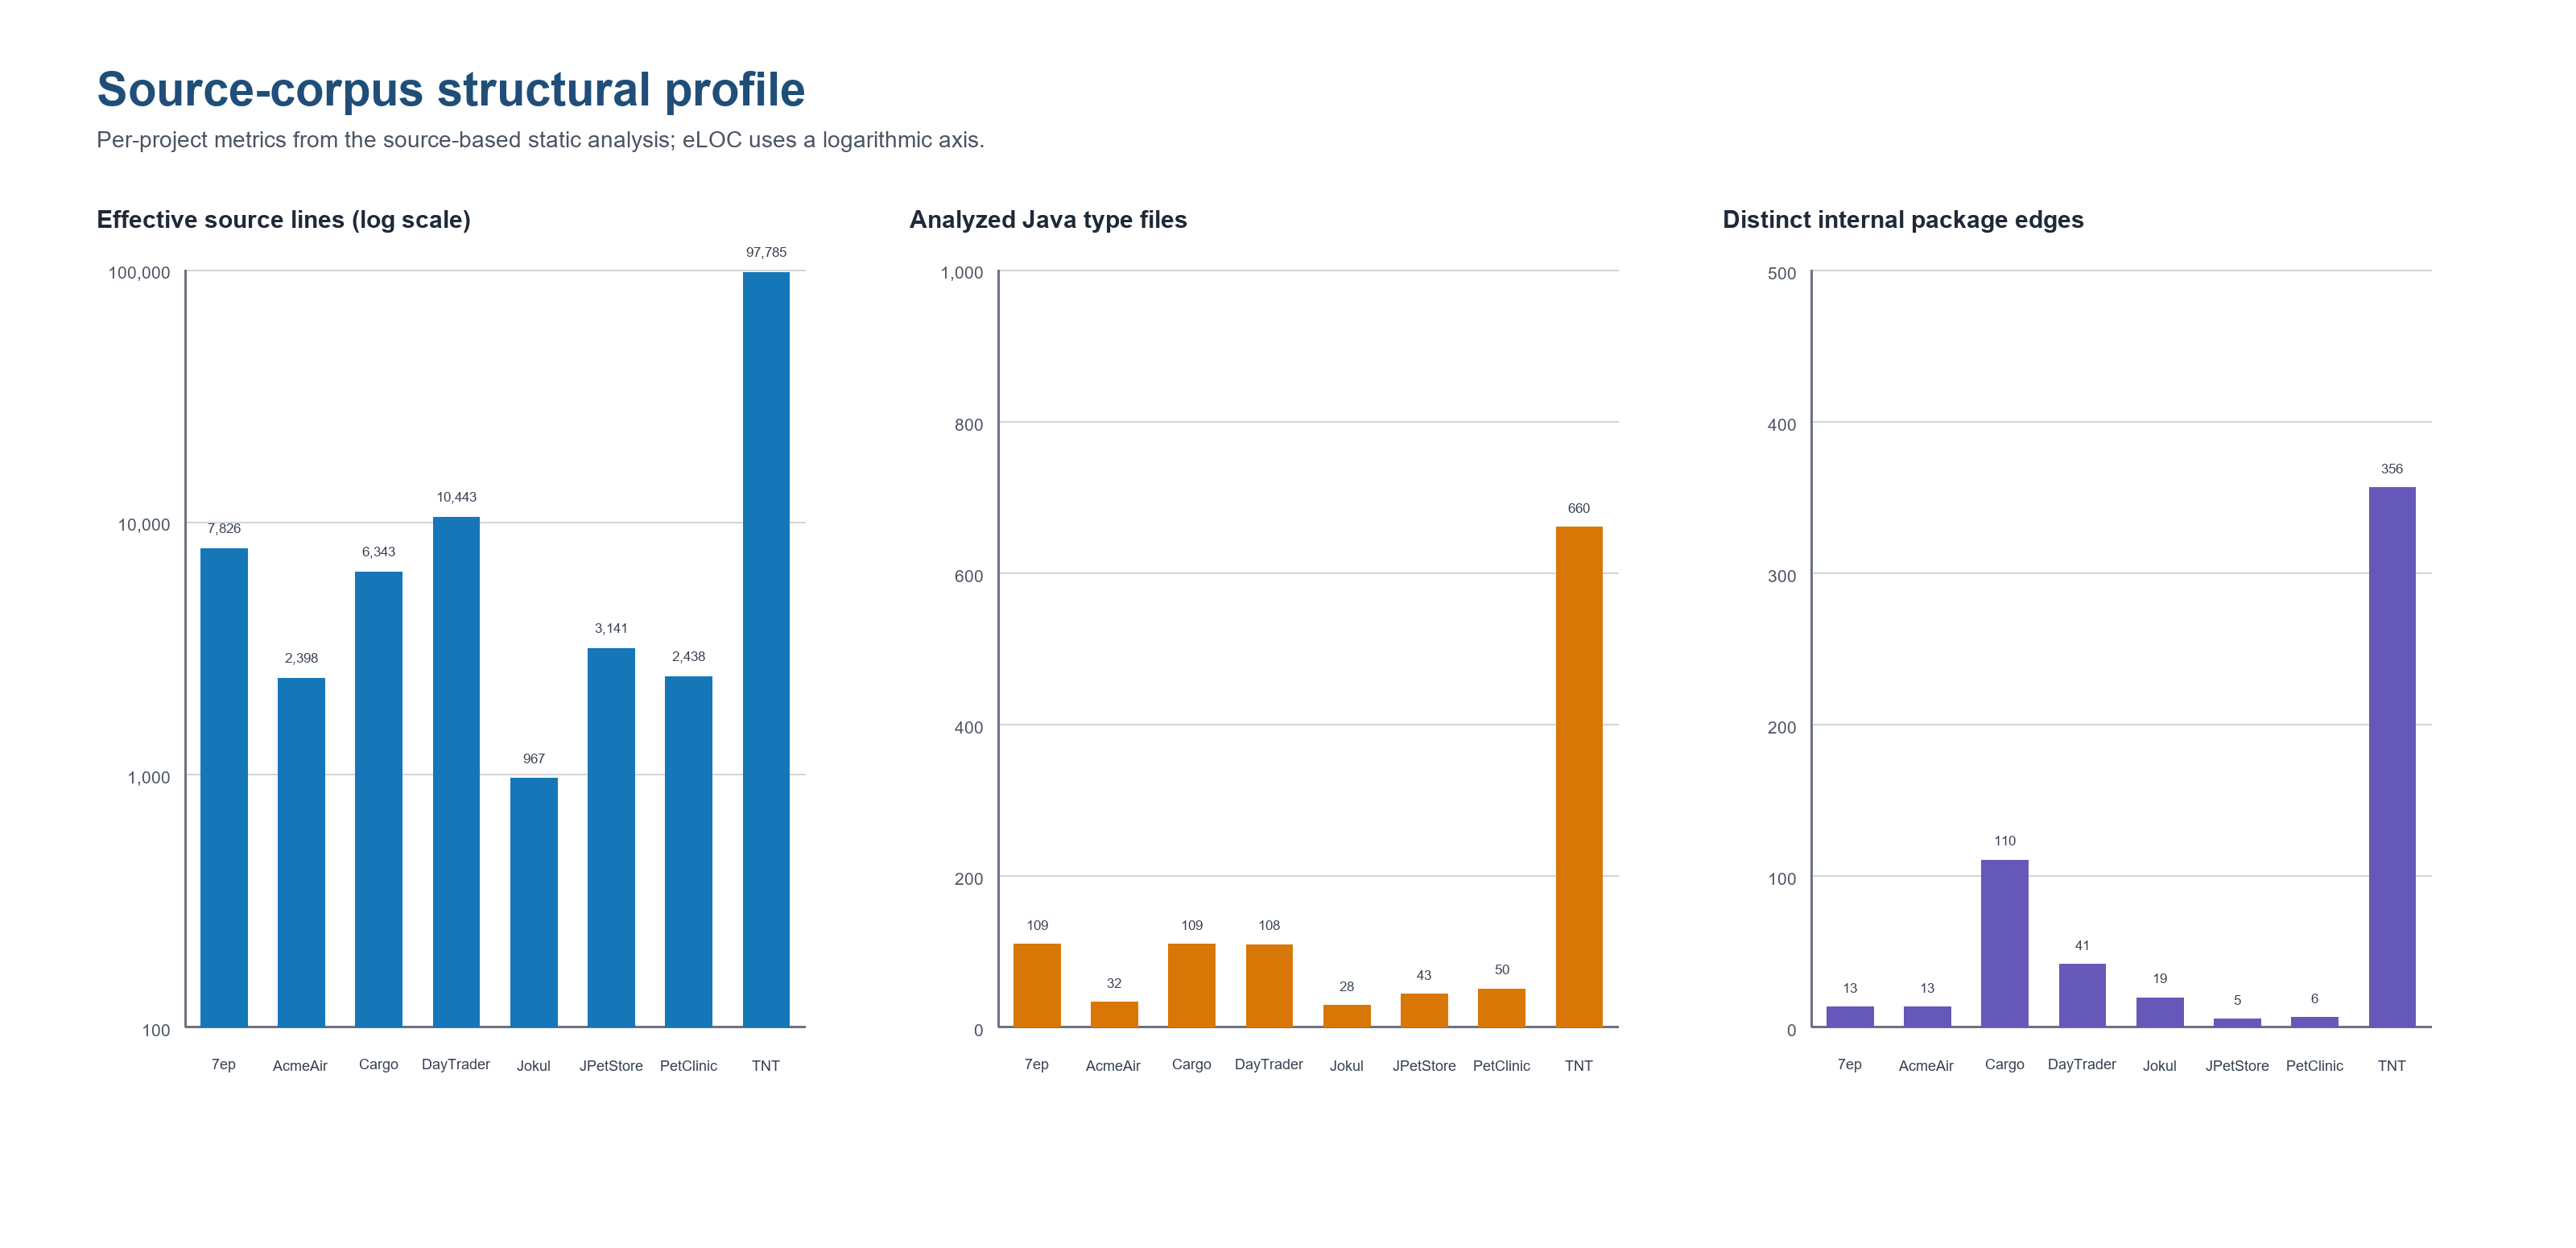
\includegraphics[width=\textwidth]{figures/fig_static_corpus_profile.png}
\caption{Static source-corpus profile. Effective source lines are shown on a logarithmic scale; package edges are distinct internal import-derived relations.}
\label{fig:static-corpus-profile}
\end{figure*}

\begin{table}[t]
\centering
\small
\resizebox{\linewidth}{!}{%
\begin{tabular}{lrrrrrrrr}
\toprule
Project & Build files & Type files & Packages & Methods & eLOC & Internal imports & Internal edges & Entrypoints \\
\midrule
7ep & 3 & 109 & 14 & 670 & 7,826 & 112 & 13 & 14 \\
acmeair & 1 & 32 & 10 & 151 & 2,398 & 38 & 13 & 8 \\
cargo-tracker & 1 & 109 & 28 & 617 & 6,343 & 355 & 110 & 5 \\
daytrader7 & 4 & 108 & 11 & 1,011 & 10,443 & 235 & 41 & 45 \\
Jokul & 1 & 28 & 12 & 119 & 967 & 45 & 19 & 5 \\
jpetstore & 1 & 43 & 6 & 366 & 3,141 & 61 & 5 & 1 \\
pet-clinic & 2 & 50 & 7 & 204 & 2,438 & 34 & 6 & 10 \\
TNTConcept & 3 & 660 & 72 & 15,401 & 97,785 & 2,691 & 356 & 0 \\
\bottomrule
\end{tabular}
}
\caption{Static source-corpus profile. Type files are analyzed Java type files; internal edges are distinct import-derived package relations.}
\label{tab:static-corpus}
\end{table}

\subsection{Structural properties of direct-generation outputs}

Across the 48 valid direct-generation outputs, the median service count was 4 (IQR 3--5), and the median number of valid directed communications was 9 (IQR 6--13). Median communication density was 0.67, while the median responsibility length was 23.8 words per service. These values summarize output structure and lexical detail; they do not establish that a larger or denser architecture is better.

\begin{table}[t]
\centering
\small
\begin{tabular}{llrrrrr}
\toprule
Provider & Prompt & n & Services & Valid links & Density & Responsibility words \\
\midrule
OpenAI & zero-shot & 8 & 3.5 [3.0, 4.0] & 6.0 [6.0, 10.0] & 0.92 [0.79, 1.00] & 31.0 [27.0, 32.9] \\
OpenAI & few-shot & 8 & 3.5 [3.0, 4.2] & 6.0 [6.0, 11.5] & 0.82 [0.71, 1.00] & 25.5 [21.9, 28.9] \\
Anthropic & zero-shot & 8 & 4.5 [3.8, 5.0] & 9.5 [5.5, 11.5] & 0.60 [0.43, 0.71] & 40.3 [33.8, 42.9] \\
Anthropic & few-shot & 8 & 4.5 [3.0, 5.2] & 9.5 [4.8, 14.2] & 0.66 [0.50, 0.73] & 23.8 [23.0, 25.1] \\
DeepSeek & zero-shot & 8 & 4.5 [4.0, 6.0] & 10.5 [6.8, 13.2] & 0.53 [0.46, 0.65] & 13.6 [9.9, 17.9] \\
DeepSeek & few-shot & 8 & 4.5 [3.8, 5.2] & 9.5 [7.0, 12.2] & 0.53 [0.42, 0.67] & 13.7 [10.8, 15.6] \\
\bottomrule
\end{tabular}
\caption{Descriptive structural statistics for valid direct-generation outputs. Entries are median [Q1, Q3] across available systems.}
\label{tab:direct-by-condition}
\end{table}

\begin{figure*}[t]
\centering
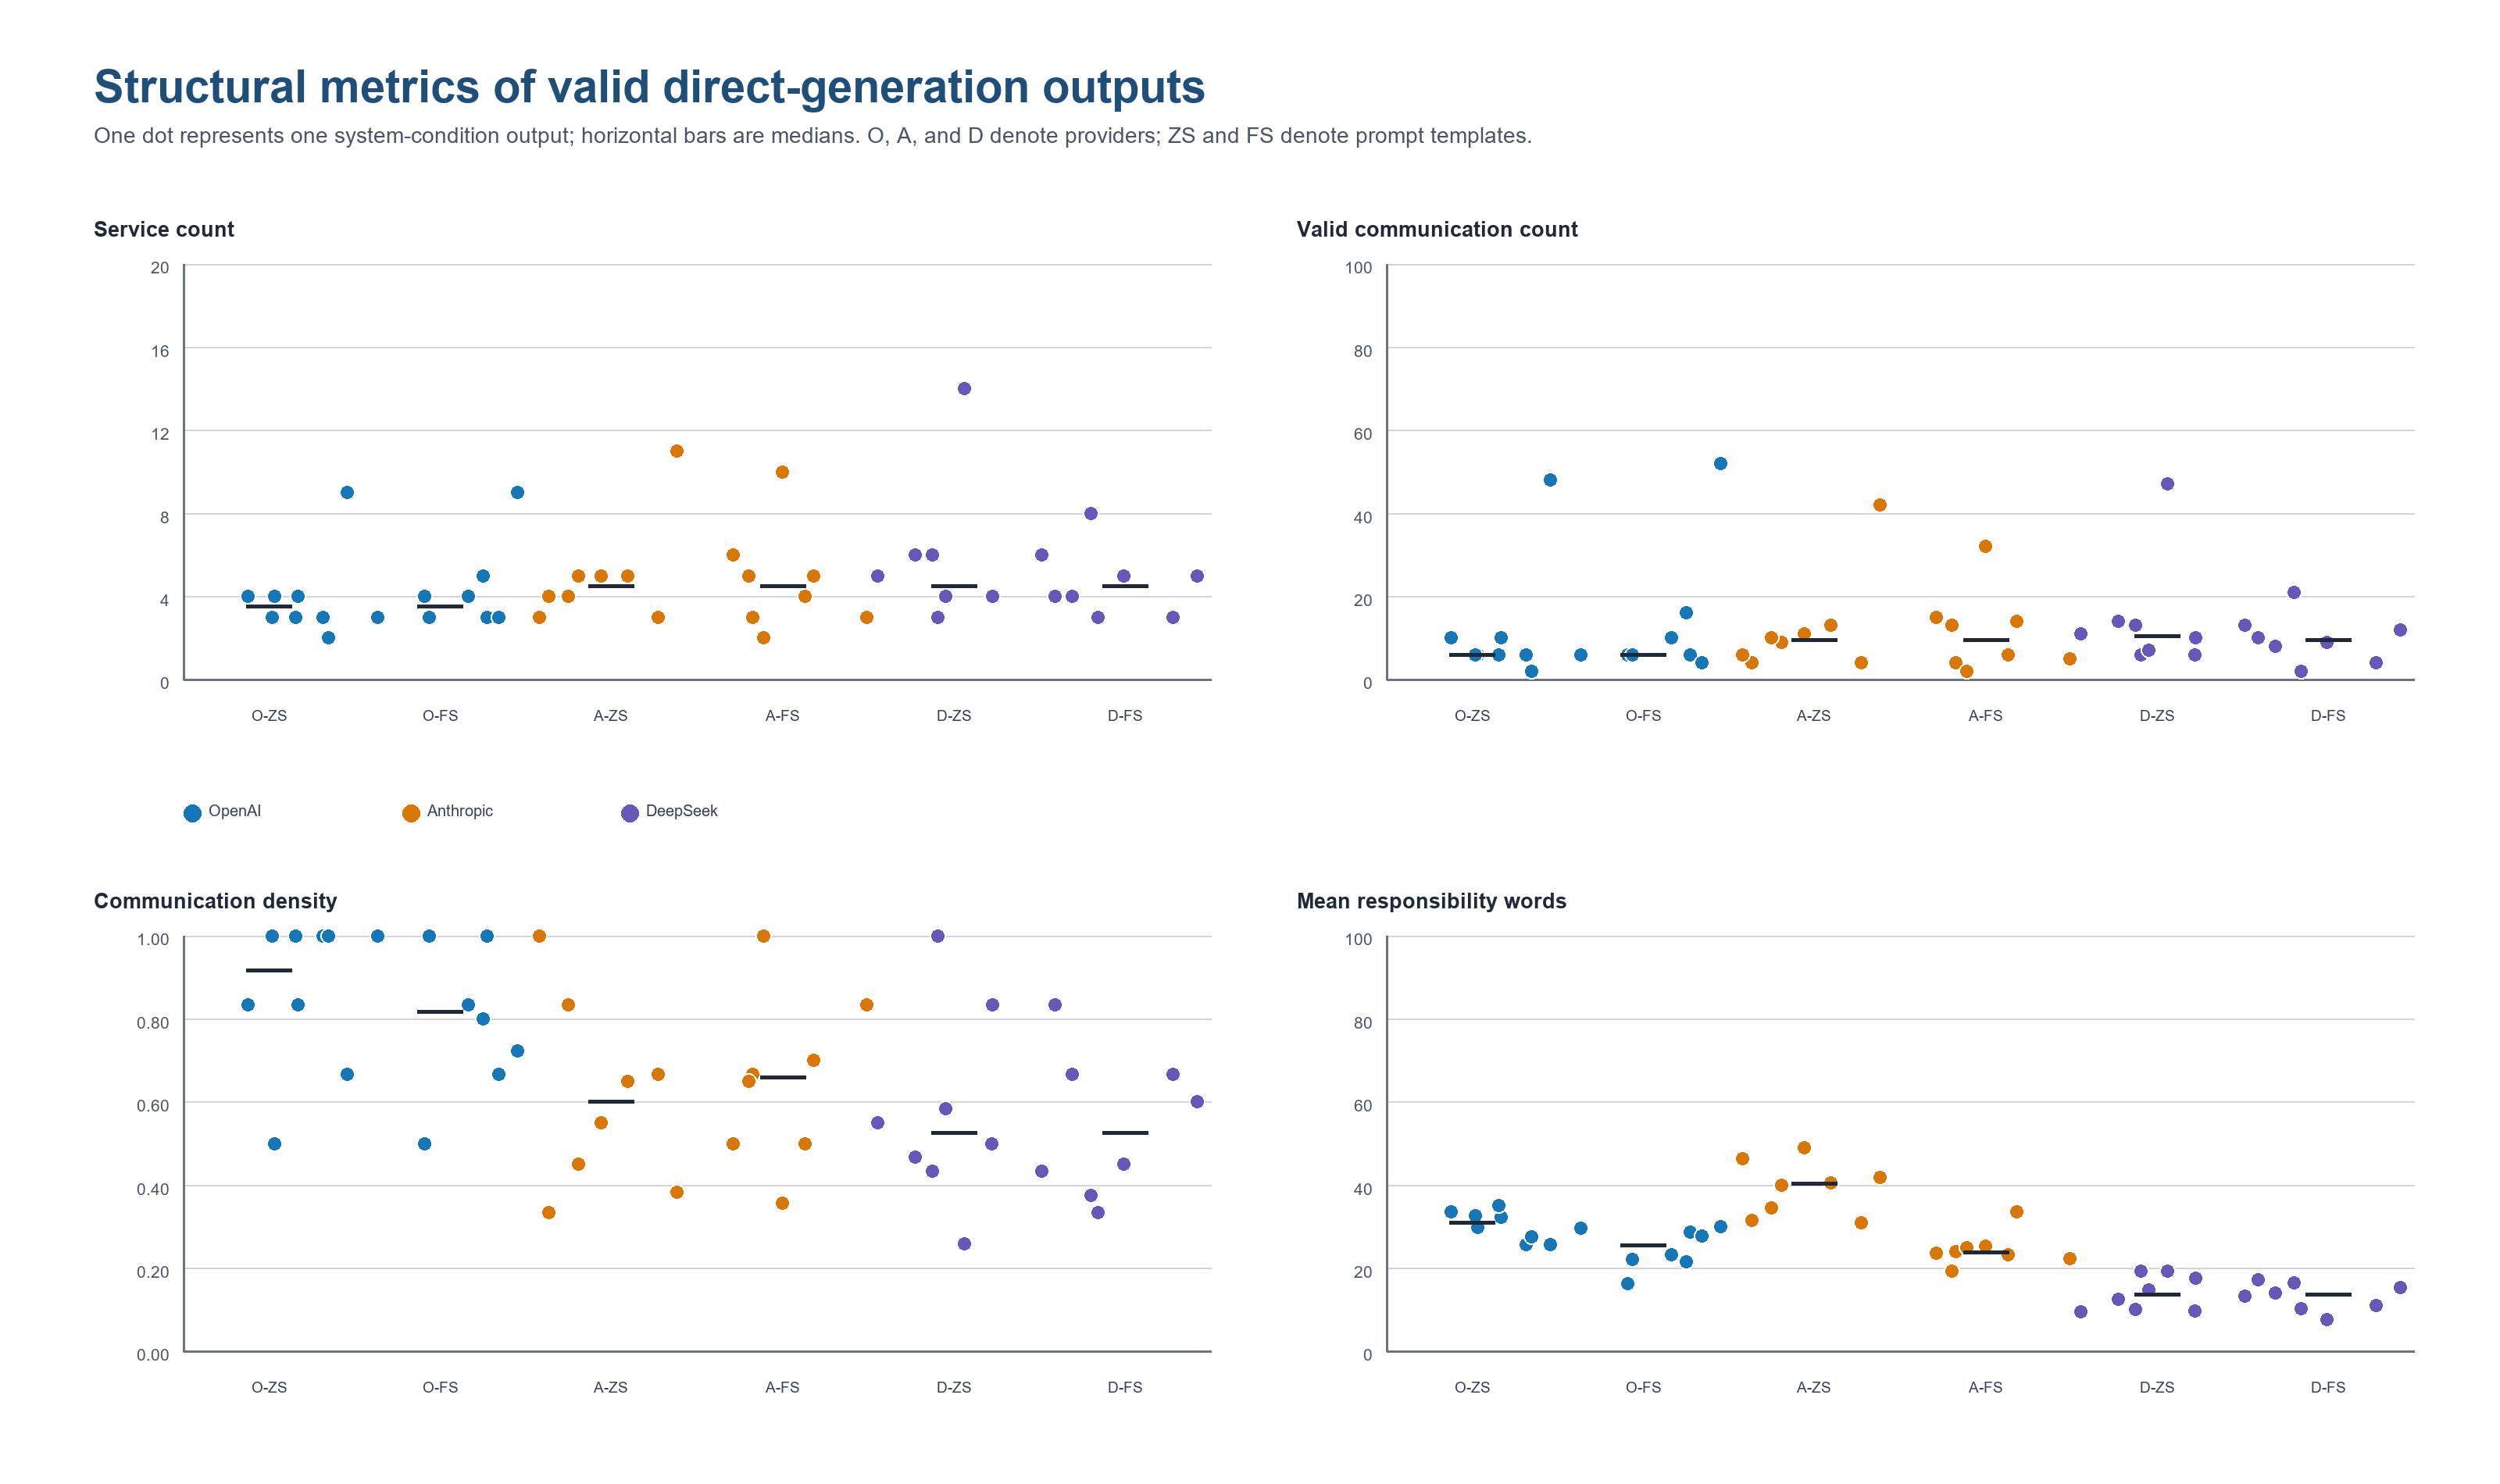
\includegraphics[width=\textwidth]{figures/fig_direct_architecture_metrics.png}
\caption{Distribution of structural metrics across valid direct-generation outputs. Each point is one system-condition output, and horizontal bars denote medians within a provider--prompt condition.}
\label{fig:direct-architecture-metrics}
\end{figure*}

\subsection{Reference-aware comparison of direct outputs}
\label{sec:reference-aware-results}

To complement the structural description, each of the 48 direct-prompt outputs was compared with the human-authored reference architecture for its project. This comparison is reference-aware rather than name-exact: a generated service could match a reference service when its responsibility had sufficient deterministic semantic similarity, even when their labels differed. The matching procedure combines service-name terms, responsibility terms, and domain-concept aliases, and then selects a one-to-one service mapping with a similarity threshold of 0.420. Thus, for example, an identity-and-access service can be aligned with an authentication service when their responsibilities describe the same capability. The complete selected mappings and scores are retained in the accompanying evaluation workbook.

Service-boundary precision, recall, and F1 were calculated from this one-to-one mapping. Directed communication metrics were then calculated after replacing generated endpoints with their matched reference services; a communication was a true positive only when the corresponding directed reference relation existed. The metrics therefore distinguish recovery of service responsibilities from recovery of the reference interaction structure. Values in Table~\ref{tab:reference-provider-metrics} are macro averages across the eight projects and the two prompt styles for each provider; they are descriptive because the snapshot contains one output per condition.

\begin{table*}[t]
\centering
\small
\begin{tabular}{lrrrrrrrrr}
\toprule
& \multicolumn{3}{c}{Service boundaries} & \multicolumn{3}{c}{Directed communications} & \multicolumn{3}{c}{Combined} \\
\cmidrule(lr){2-4}\cmidrule(lr){5-7}\cmidrule(lr){8-10}
Provider & Precision & Recall & F1 & Precision & Recall & F1 & Precision & Recall & F1 \\
\midrule
DeepSeek & 0.832 & 0.706 & 0.754 & 0.341 & 0.439 & 0.373 & 0.513 & 0.541 & 0.511 \\
OpenAI   & 0.970 & 0.639 & 0.760 & 0.398 & 0.420 & 0.381 & 0.586 & 0.503 & 0.518 \\
Claude   & 0.891 & 0.686 & 0.766 & 0.382 & 0.440 & 0.400 & 0.565 & 0.536 & 0.537 \\
\bottomrule
\end{tabular}
\caption{Reference-aware metrics for direct-prompt outputs. Values are macro means over eight projects and the zero-shot and few-shot outputs for each provider. ``Combined'' pools service and directed-communication decisions; it is reported as a compact summary, while the separate service and communication columns should be interpreted independently.}
\label{tab:reference-provider-metrics}
\end{table*}

At the aggregate level, service-boundary F1 was similar across providers (0.754--0.766), whereas directed-communication F1 was substantially lower (0.373--0.400). This pattern indicates that responsibility-oriented service boundaries were more often aligned with the reference than the exact directed interaction structures. Claude obtained the largest combined macro F1 (0.537), followed by OpenAI (0.518) and DeepSeek (0.511); the small descriptive differences should not be interpreted as inferential evidence of provider superiority.

Table~\ref{tab:reference-project-f1} details the variation by project. Each entry is the mean F1 over the zero-shot and few-shot direct outputs. The large variation across projects is visible in both service and communication recovery: for example, all providers obtained service F1 of 1.000 for Jokul, whereas directed-communication F1 for 7ep ranged from 0.000 to 0.167. The communication results for PetClinic also varied markedly, including zero F1 for both Claude conditions under the reference-directed relation criterion.

\begin{table*}[t]
\centering
\footnotesize
\resizebox{\textwidth}{!}{%
\begin{tabular}{lrrrrrrrrr}
\toprule
& \multicolumn{3}{c}{DeepSeek} & \multicolumn{3}{c}{OpenAI} & \multicolumn{3}{c}{Claude} \\
\cmidrule(lr){2-4}\cmidrule(lr){5-7}\cmidrule(lr){8-10}
Project & Service F1 & Communication F1 & Combined F1 & Service F1 & Communication F1 & Combined F1 & Service F1 & Communication F1 & Combined F1 \\
\midrule
7ep           & 0.382 & 0.000 & 0.152 & 0.636 & 0.167 & 0.345 & 0.455 & 0.056 & 0.215 \\
AcmeAir       & 0.780 & 0.202 & 0.421 & 0.855 & 0.514 & 0.629 & 0.909 & 0.745 & 0.804 \\
Cargo Tracker & 0.700 & 0.409 & 0.500 & 0.667 & 0.444 & 0.519 & 0.727 & 0.420 & 0.515 \\
DayTrader7    & 0.750 & 0.493 & 0.573 & 0.800 & 0.435 & 0.545 & 0.871 & 0.632 & 0.703 \\
Jokul         & 1.000 & 0.619 & 0.785 & 1.000 & 0.667 & 0.800 & 1.000 & 0.619 & 0.785 \\
JPetStore     & 0.909 & 0.438 & 0.603 & 0.667 & 0.267 & 0.417 & 0.733 & 0.353 & 0.493 \\
PetClinic     & 0.875 & 0.515 & 0.663 & 0.762 & 0.250 & 0.500 & 0.619 & 0.000 & 0.300 \\
TNTConcept    & 0.640 & 0.307 & 0.394 & 0.696 & 0.306 & 0.386 & 0.815 & 0.371 & 0.481 \\
\bottomrule
\end{tabular}}
\caption{Reference-aware F1 by project and provider. Each cell is the mean across that provider's zero-shot and few-shot direct outputs. Service and communication F1 use different matching objects; combined F1 pools their decisions.}
\label{tab:reference-project-f1}
\end{table*}

Figure~\ref{fig:reference-aware-project-f1} visualizes the same project-level results and makes the gap between service-boundary and directed-communication recovery apparent. AcmeAir and Jokul show comparatively high alignment for multiple providers, while 7ep and PetClinic show particularly low recovery of the specified directed communication relations. The figure should be read as a comparison to the reviewed reference baseline, not as evidence that alternative architectures are necessarily incorrect.

\begin{figure*}[t]
\centering
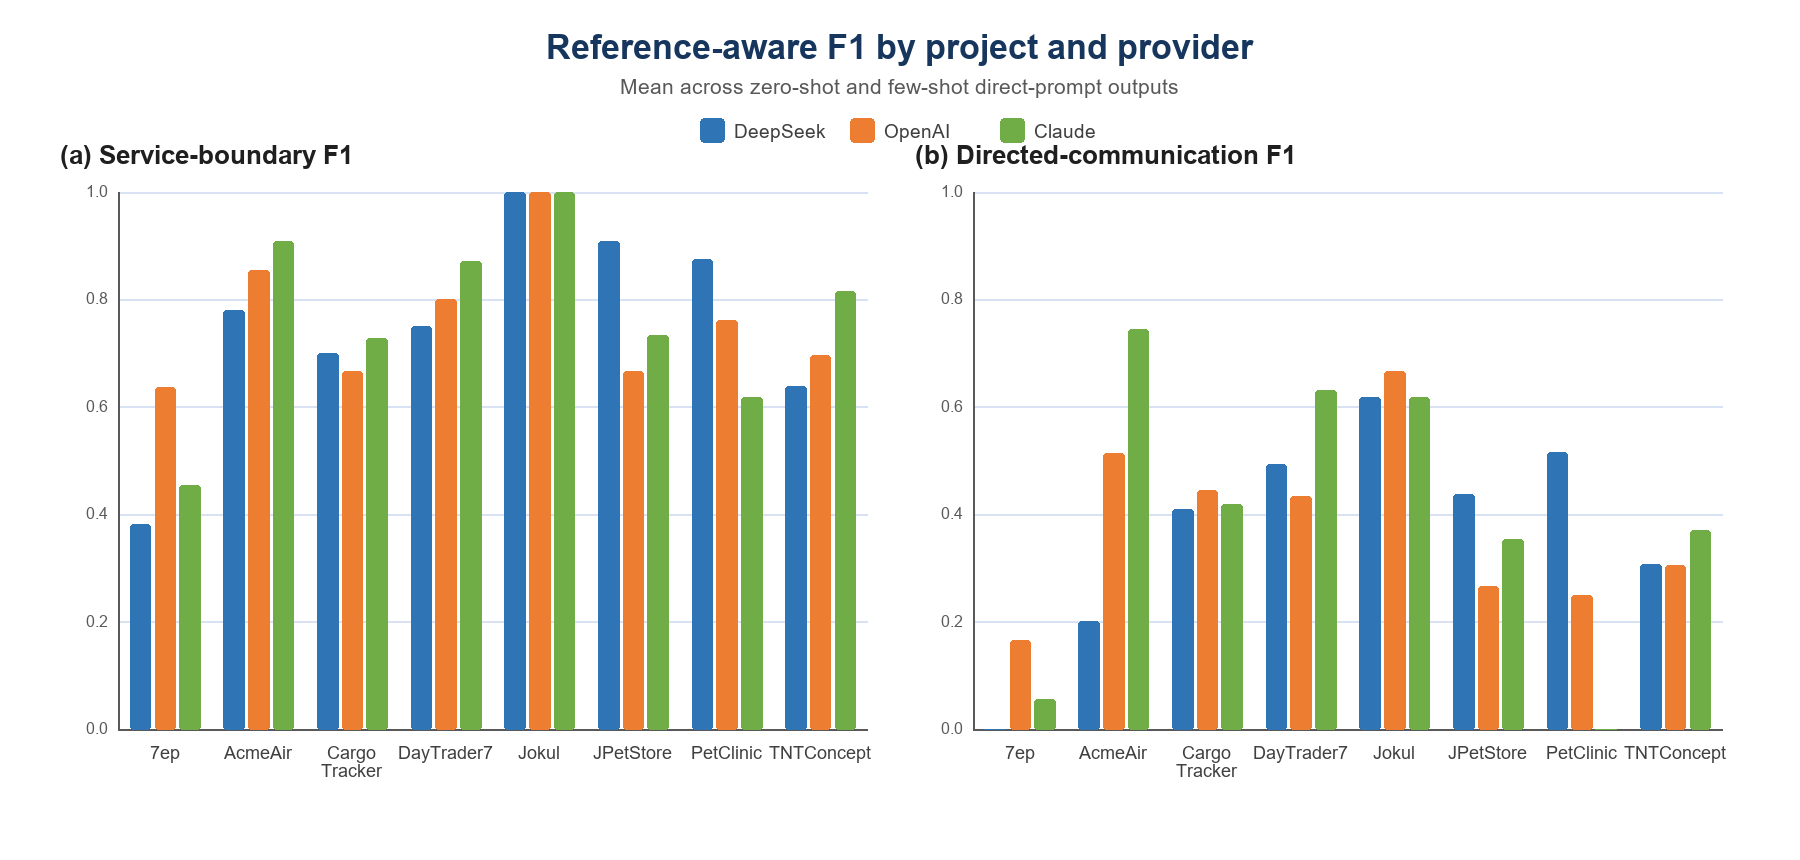
\includegraphics[width=\textwidth]{figures/fig_reference_aware_project_f1.png}
\caption{Reference-aware F1 by project and provider. Bars are means across zero-shot and few-shot direct-prompt outputs. Panel (a) evaluates one-to-one responsibility-aware service matches; panel (b) evaluates directed communications after their endpoints are translated through those service matches.}
\label{fig:reference-aware-project-f1}
\end{figure*}

\subsection{Interpretation boundary}

The reported measures are deliberately descriptive. Structural regularity, prompt volume, and trace duration are useful audit signals. The reference-aware scores additionally quantify alignment with the reviewed reference baseline under the stated semantic matching rule, but they do not establish that a different decomposition is invalid, nor do they independently demonstrate requirement coverage, domain correctness, implementability, or provider superiority. Those claims require the planned expert-review data and, where appropriate, independent architectural validation.

\section{Discussion}
\subsection{Comparison between Agent-Based and Direct Prompting}
\subsection{Implications for Researchers and Practitioners}
\subsection{Methodology for LLM-Assisted Architecture Transformation}

\section{Threats to Validity}

\section{Conclusion}

\end{document}
\endinput
%%
%% End of file `acmsmall-submission.tex'.
